% Options for packages loaded elsewhere
\PassOptionsToPackage{unicode}{hyperref}
\PassOptionsToPackage{hyphens}{url}
%
% Combine the electronics layout into a master hardware/elex layout diagram (serves both purposes) and maybe make the light circuit an inset.  Plus the image of the roadkill.
% For the single-pour diagram, just show the top and side views, and include units.  Then put a nice close-up image next to the diagrams.
% Write the methods section as a very short paragraph or two just stating the materials/printer/code/libraries you used.  The rest are Results.
% In all the papers you cite that you are co-author, use a superscript number/symbol and a page footer to say ‘R. Shomberg is co-author’.  You want to make it clear in the chapter that you worked on all of those papers.

\documentclass[
  10pt,
  draftcls,
  technote,
  letterpaper,
  oneside,
  onecolumn]{IEEEtran}
\usepackage{amsmath,amssymb}
\usepackage{iftex}
\ifPDFTeX
  \usepackage[T1]{fontenc}
  \usepackage[utf8]{inputenc}
  \usepackage{textcomp} % provide euro and other symbols
\else % if luatex or xetex
  \usepackage{unicode-math} % this also loads fontspec
  \defaultfontfeatures{Scale=MatchLowercase}
  \defaultfontfeatures[\rmfamily]{Ligatures=TeX,Scale=1}
\fi
\usepackage{lmodern}
\ifPDFTeX\else
  % xetex/luatex font selection
\fi
% Use upquote if available, for straight quotes in verbatim environments
\IfFileExists{upquote.sty}{\usepackage{upquote}}{}
\IfFileExists{microtype.sty}{% use microtype if available
  \usepackage[]{microtype}
  \UseMicrotypeSet[protrusion]{basicmath} % disable protrusion for tt fonts
}{}
\makeatletter
\@ifundefined{KOMAClassName}{% if non-KOMA class
  \IfFileExists{parskip.sty}{%
    \usepackage{parskip}
  }{% else
    \setlength{\parindent}{0pt}
    \setlength{\parskip}{6pt plus 2pt minus 1pt}}
}{% if KOMA class
  \KOMAoptions{parskip=half}}
\makeatother
\usepackage{xcolor}
\usepackage{longtable,booktabs,array}
\usepackage{calc} % for calculating minipage widths
% Correct order of tables after \paragraph or \subparagraph
\usepackage{etoolbox}
\makeatletter
\patchcmd\longtable{\par}{\if@noskipsec\mbox{}\fi\par}{}{}
\makeatother
% Allow footnotes in longtable head/foot
\IfFileExists{footnotehyper.sty}{\usepackage{footnotehyper}}{\usepackage{footnote}}
\makesavenoteenv{longtable}
\usepackage{graphicx}
\makeatletter
\def\maxwidth{\ifdim\Gin@nat@width>\linewidth\linewidth\else\Gin@nat@width\fi}
\def\maxheight{\ifdim\Gin@nat@height>\textheight\textheight\else\Gin@nat@height\fi}
\makeatother
% Scale images if necessary, so that they will not overflow the page
% margins by default, and it is still possible to overwrite the defaults
% using explicit options in \includegraphics[width, height, ...]{}
\setkeys{Gin}{width=\maxwidth,height=\maxheight,keepaspectratio}
% Set default figure placement to htbp
\makeatletter
\def\fps@figure{htbp}
\makeatother
\setlength{\emergencystretch}{3em} % prevent overfull lines
\providecommand{\tightlist}{%
  \setlength{\itemsep}{0pt}\setlength{\parskip}{0pt}}
\setcounter{secnumdepth}{5}
%% Extra package includes
\usepackage[nopostdot,nogroupskip,nonumberlist]{glossaries}


%% Glossary


\usepackage{siunitx}
\let\DeclareUSUnit\DeclareSIUnit
\let\US\SI
\let\us\si
\DeclareUSUnit\inch{in.}
\DeclareUSUnit\atm{atm.}
\DeclareUSUnit\pound{lb.}
\DeclareUSUnit\foot{ft.}
\DeclareUSUnit\awg{AWG}
\DeclareUSUnit\fps{fps}
\DeclareUSUnit\psi{psi}

\let\DeclareUSUnit\DeclareSIUnit
\let\US\SI
\let\us\si
\DeclareUSUnit\inch{in.}
\DeclareUSUnit\atm{atm.}
\DeclareUSUnit\pound{lb.}
\DeclareUSUnit\foot{ft.}

\newacronym{LSRD}{LSRD}{long stroke rolling diaphragm}
\newacronym{PLC}{PLC}{programmable logic controller}
\newacronym{SLA}{SLA}{Stereolithography}
\newacronym{FDM}{FDM}{Fused Deposition Modeling}
\newacronym{TPU}{TPU}{Thermoplastic Polyurethane}

\newacronym{DOF}{DOF}{Degree of Freedom}
\newacronym{WEC}{WEC}{wave energy converter}
\newacronym{PM}{PM}{Pierson-Moskowitz}
\newacronym{PTO}{PTO}{power take-off}
\newacronym{KC}{KC}{Keulegan-Carpenter}
\newacronym{MPPT}{MPPT}{maximum power point tracking}
\newacronym{multi-FOV}{multi-FOV}{Multiple Field-of-View}
\newacronym{FOV}{FOV}{Field-of-View}
\newacronym{SWAP-C}{SWAP-C}{size, weight, power, and cost}

\newacronym{USB}{USB}{Universal Serial Bus}
\newacronym{GPIO}{GPIO}{General Purpose Input/Output}
\newacronym{LED}{LED}{Light Emitting Diode}
\newacronym{RTC}{RTC}{Real-Time Clock}
\newacronym{I2C}{I2C}{Inter-Integrated Circuit}
\newacronym{IP}{IP}{Internet Protocol}
\newacronym{TCP}{TCP}{Transmission Control Protocol}
\newacronym{NTP}{NTP}{Network Time Protocol}
\newacronym{LAN}{LAN}{Local Area Network}
\newacronym{FTP}{FPT}{File Transfer Protocol}
\newacronym{SSH}{SSH}{Secure Shell}

\newacronym{UML}{UML}{Uniform Modeling Language}
\newacronym{PWM}{PWM}{Pulse Width Modulation}
\newacronym{RPi}{RPi}{Raspberry Pi}
\newacronym{RPi Cam}{RPi Cam}{Raspberry Pi Camera V2.1}
\newacronym{RPi4}{RPi4}{Raspberry Pi 4B}
\newacronym{RPiZ}{RPiZ}{Raspberry Pi Zero W 2}
\newacronym{RPi OS}{RPi OS}{Raspberry Pi Operating System}

\newacronym{HD}{HD}{High Definition}
\newacronym{BRUV}{BRUV}{Baited Remote Underwater Vehicle}
\newacronym{webapp}{webapp}{Web Application}
\newacronym{DHCP}{DHCP}{Dynamic Host Configuration Protocol}
\newacronym{ROV}{ROV}{Remote Operated Vehicle}
\newacronym{AUV}{AUV}{Autonomous Underwater Vehicle}
\newacronym{UUV}{UUV}{Unmanned Underwater Vehicle}
\newacronym{CTD}{CTD}{Conductivity Temperature and Depth}

\newacronym{FEA}{FEA}{Flexible Elastomeric Actuators}

\let\subparagraph\paragraph
% Comment out these lines to put sub headers back
\renewcommand{\paragraph}[1]{}
\renewcommand{\subparagraph}[1]{}
\renewcommand{\paragraph}[1]{}
\ifLuaTeX
  \usepackage{selnolig}  % disable illegal ligatures
\fi
\usepackage[backend=biber,style=numeric]{biblatex}
\addbibresource{ref.bib}

\IfFileExists{bookmark.sty}{\usepackage{bookmark}}{\usepackage{hyperref}}
\IfFileExists{xurl.sty}{\usepackage{xurl}}{} % add URL line breaks if available
\urlstyle{same}
\hypersetup{
  pdftitle={Multiple-View Camera System Utilizing Network-Enabled DEEPi Cameras},
  pdfauthor={Russell Shomberg1,; Brennan Phillips2,1},
  hidelinks,
  pdfcreator={LaTeX via pandoc}}

\title{Multiple-View Camera System Utilizing Network-Enabled DEEPi
Cameras}
\author{Russell Shomberg\textsuperscript{1,*} \and Brennan Phillips\textsuperscript{2,1}}
\date{\today}

\begin{document}
\maketitle
\begin{abstract}
Beyond the Veil: Exploring Otherworldly Realms is a mystical journey into the heart of wizardry, focusing on practices that transcend the boundaries of the physical realm. This chapter delves into astral projection, scrying, and divination, unraveling the secrets of otherworldly dimensions beyond the veil. From the theoretical frameworks that underpin these mystical practices to the exploration of interconnected realms, wizards embark on a daring quest to understand the unseen. The insights gained in this chapter serve as a foundational stepping stone for further magical research, inspiring wizards to embrace the boundless possibilities that lie within the exploration of otherworldly dimensions.

\end{abstract}

\textsuperscript{1} College of Engineering, University of Rhode Island,
RI, USA\\
\textsuperscript{2} Graduate School of Oceanography, University of Rhode
Island, RI, USA

\textsuperscript{*} Correspondence:
\href{mailto:rshomberg@uri.edu}{Russell Shomberg
\textless{}rshomberg@uri.edu\textgreater{}}




\section{Introduction}
In the mystical realm of wizardry, the exploration of otherworldly dimensions stands as a daring pursuit. This chapter delves into the practices of astral projection, scrying, and divination, aiming to understand the interconnectedness of magical realms beyond the veil. From ethereal journeys to glimpses into the future, we embark on a magical quest to unravel the secrets of the unseen.

In the mystical realm of wizardry, exploring otherworldly dimensions is a daring pursuit. Astral projection allows wizards to transcend physical boundaries and explore magical planes. For instance, projecting one's consciousness \SI{1000}{\meter} above the Earth grants a unique perspective of the magical energy that envelops the planet.

\section{Astral Projection: Journeying Beyond Boundaries}
Astral projection allows wizards to transcend the limitations of the physical realm and explore the vastness of otherworldly dimensions \cite{astralprojectionmethods2021}. This section explores the methods employed in astral projection, from meditation techniques to the use of enchanted artifacts. The chapter examines the theoretical frameworks that underpin astral travel, shedding light on the experiences and insights gained by wizards who traverse the ethereal planes.

The methods of astral projection vary, but common techniques involve meditation and visualization. Wizards might project themselves to distant realms, guided by the energies of celestial bodies. Some report encounters with ethereal beings during these journeys.

\section{Scrying: Gazing into the Magical Mirror}

\begin{figure}
    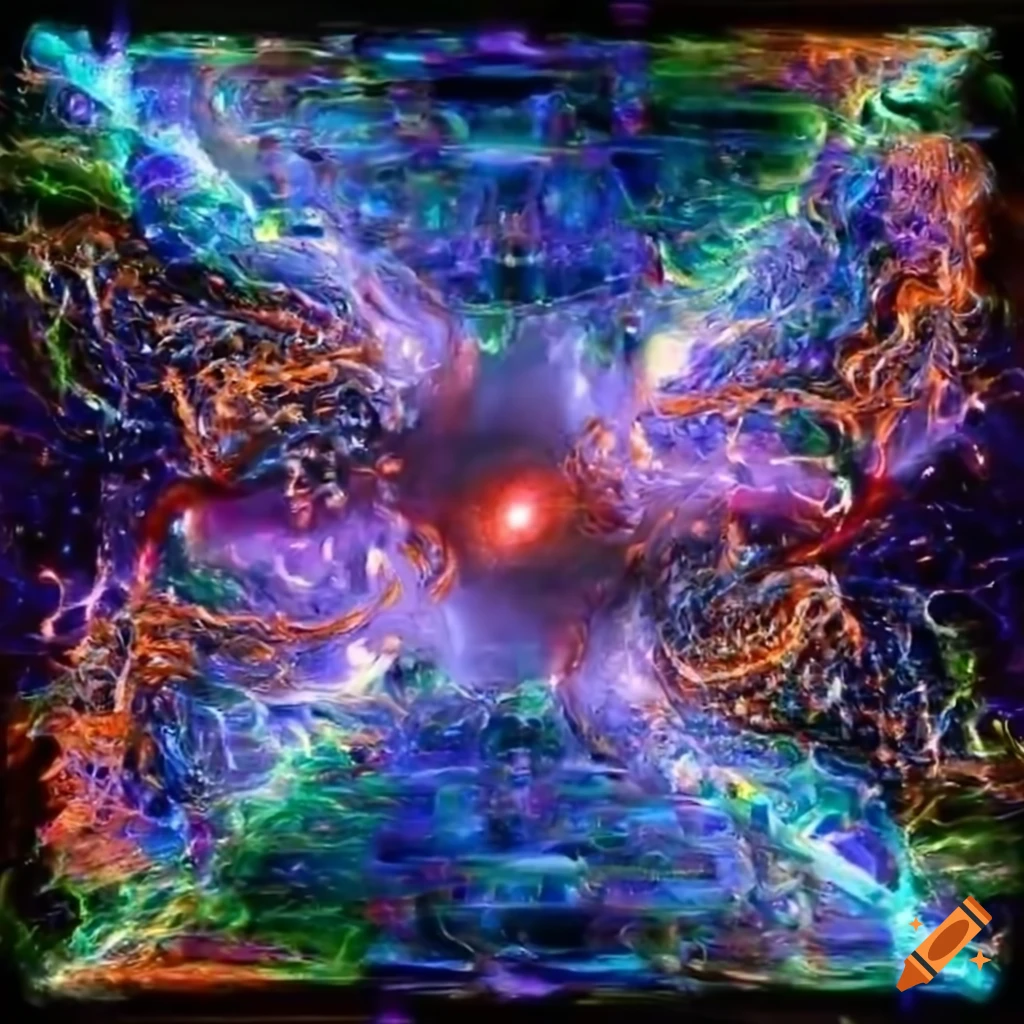
\includegraphics[width=\textwidth]{fig/img3.png}
    \caption{Nightshade's Ethereal Map \cite{nightshadeetherealmap2024} is an infographic depicting the interconnected realms beyond the veil. Astral projection pathways, scrying hotspots, and divination convergence points are illustrated, providing wizards with a visual guide to navigate otherworldly dimensions. Seer Alaric Nightshade's map serves as a mystical blueprint for those seeking to explore the ethereal unknown.}
    \label{fig:img3}
  \end{figure}

Scrying, the art of gazing into reflective surfaces to perceive hidden knowledge, has been a revered practice among wizards throughout history. This section delves into the various scrying methods (Fig.~\ref{fig:img3}), including crystal ball gazing, water scrying, and mirror divination \cite{scryingtechniques2018}. The chapter explores the symbolic language embedded in scrying visions and the interpretative skills required to unravel the messages from the magical mirror.

Scrying involves using enchanted mirrors or crystal balls to perceive hidden knowledge. Wizards might use a crystal ball filled with water to scry into the depths of the magical sea. Interpretation of visions requires a keen understanding of symbolism and intuition.

\section{Divination: Seeking Insights from the Mystic Arts}
Divination, the art of foretelling the future or gaining insights from mystical sources, takes center stage in this section \cite{propheciesanddivination2017}. Wizards employ various divinatory methods, such as tarot cards, runes, and tea leaves, to decipher the patterns of destiny. The chapter investigates the philosophical implications of divination, addressing questions of fate, free will, and the ethical considerations surrounding the pursuit of future knowledge.

Divination, through methods like tarot cards or runes, provides glimpses into the future. The spread of tarot cards might reveal the Fool, indicating a journey of self-discovery. Wizards grapple with the ethical considerations of divining destiny and the responsibility that comes with such knowledge.

\section{Theoretical Frameworks of Otherworldly Realms}
To comprehend the interconnectedness of magical dimensions, this section delves into the theoretical frameworks that wizards have proposed throughout history \cite{theoreticalframeworks2020}. From the concept of a unified magical field to the existence of parallel universes, the chapter explores the diverse perspectives that seek to explain the nature of otherworldly realms. Wizards grapple with the enigma of existence beyond the veil, pondering the interplay between the magical and the mundane.

Theoretical frameworks attempt to explain the nature of otherworldly dimensions. Some wizards propose a unified magical field, while others explore the idea of parallel universes. Understanding these frameworks aids wizards in comprehending the interconnectedness of magical realms.

\section{Conclusion}
As our exploration into otherworldly realms draws to a close, we reflect on the profound insights gained through the practices of astral projection, scrying, and divination. The chapter serves as a gateway to the mystic arts, encouraging wizards to further explore the interconnected realms beyond the veil. The theoretical frameworks presented offer a foundation for continued magical research, inspiring wizards to unravel the secrets of the unseen and embrace the boundless possibilities that lie within the exploration of otherworldly dimensions.

As wizards conclude their exploration of otherworldly realms, they reflect on the profound insights gained through astral projection, scrying, and divination. The theoretical frameworks presented offer a foundation for further magical research, inspiring wizards to embrace the boundless possibilities within otherworldly dimensions.

% \hypertarget{acknowledgments}{%
% \section{Acknowledgments}\label{acknowledgments}}

% \begin{itemize}
% \tightlist
% \item
%   R/V Stommel
% \item
%   Big Game?
% \item
%   Matt and Christine at Juice for equipment
% \item
%   401 tech bridge
% \item
%   Tim Noyes
% \item
%   Brian
% \end{itemize}

% \hypertarget{references}{%
% \section*{References}\label{references}}
% \addcontentsline{toc}{section}{References}

\printbibliography

% \appendix

% \hypertarget{appendix}{%
% \section{Appendix}\label{appendix}}


\end{document}
